% This must be in the first 5 lines to tell arXiv to use pdfLaTeX, which is strongly recommended.
\pdfoutput=1
% In particular, the hyperref package requires pdfLaTeX in order to break URLs across lines.

\documentclass[11pt]{article}\usepackage[]{graphicx}\usepackage[]{color}
% maxwidth is the original width if it is less than linewidth
% otherwise use linewidth (to make sure the graphics do not exceed the margin)
\makeatletter
\def\maxwidth{ %
  \ifdim\Gin@nat@width>\linewidth
    \linewidth
  \else
    \Gin@nat@width
  \fi
}
\makeatother

\definecolor{fgcolor}{rgb}{0.345, 0.345, 0.345}
\newcommand{\hlnum}[1]{\textcolor[rgb]{0.686,0.059,0.569}{#1}}%
\newcommand{\hlstr}[1]{\textcolor[rgb]{0.192,0.494,0.8}{#1}}%
\newcommand{\hlcom}[1]{\textcolor[rgb]{0.678,0.584,0.686}{\textit{#1}}}%
\newcommand{\hlopt}[1]{\textcolor[rgb]{0,0,0}{#1}}%
\newcommand{\hlstd}[1]{\textcolor[rgb]{0.345,0.345,0.345}{#1}}%
\newcommand{\hlkwa}[1]{\textcolor[rgb]{0.161,0.373,0.58}{\textbf{#1}}}%
\newcommand{\hlkwb}[1]{\textcolor[rgb]{0.69,0.353,0.396}{#1}}%
\newcommand{\hlkwc}[1]{\textcolor[rgb]{0.333,0.667,0.333}{#1}}%
\newcommand{\hlkwd}[1]{\textcolor[rgb]{0.737,0.353,0.396}{\textbf{#1}}}%
\let\hlipl\hlkwb

\usepackage{framed}
\makeatletter
\newenvironment{kframe}{%
 \def\at@end@of@kframe{}%
 \ifinner\ifhmode%
  \def\at@end@of@kframe{\end{minipage}}%
  \begin{minipage}{\columnwidth}%
 \fi\fi%
 \def\FrameCommand##1{\hskip\@totalleftmargin \hskip-\fboxsep
 \colorbox{shadecolor}{##1}\hskip-\fboxsep
     % There is no \\@totalrightmargin, so:
     \hskip-\linewidth \hskip-\@totalleftmargin \hskip\columnwidth}%
 \MakeFramed {\advance\hsize-\width
   \@totalleftmargin\z@ \linewidth\hsize
   \@setminipage}}%
 {\par\unskip\endMakeFramed%
 \at@end@of@kframe}
\makeatother

\definecolor{shadecolor}{rgb}{.97, .97, .97}
\definecolor{messagecolor}{rgb}{0, 0, 0}
\definecolor{warningcolor}{rgb}{1, 0, 1}
\definecolor{errorcolor}{rgb}{1, 0, 0}
\newenvironment{knitrout}{}{} % an empty environment to be redefined in TeX

\usepackage{alltt}

% Remove the "review" option to generate the final version.
\usepackage{acl} % [review]{acl}

% Standard package includes
\usepackage{times}
\usepackage{latexsym}
\usepackage[normalem]{ulem}

% For proper rendering and hyphenation of words containing Latin characters (including in bib files)
\usepackage[T1]{fontenc}
% For Vietnamese characters
% \usepackage[T5]{fontenc}
% See https://www.latex-project.org/help/documentation/encguide.pdf for other character sets

% This assumes your files are encoded as UTF8
\usepackage[utf8]{inputenc}

% This is not strictly necessary, and may be commented out,
% but it will improve the layout of the manuscript,
% and will typically save some space.
\usepackage{microtype}

\usepackage{gb4e}\noautomath
\usepackage{amsmath}\noautomath

\usepackage[edges]{forest}

\def\citeapos#1{\citeauthor{#1}'s (\citeyear{#1})} 

% If the title and author information does not fit in the area allocated, uncomment the following
%
%\setlength\titlebox{<dim>}
%
% and set <dim> to something 5cm or larger.

\title{A multinomial processing tree model of RC attachment}

% Author information can be set in various styles:
% For several authors from the same institution:
% \author{Author 1 \and ... \and Author n \\
%         Address line \\ ... \\ Address line}
% if the names do not fit well on one line use
%         Author 1 \\ {\bf Author 2} \\ ... \\ {\bf Author n} \\
% For authors from different institutions:
% \author{Author 1 \\ Address line \\  ... \\ Address line
%         \And  ... \And
%         Author n \\ Address line \\ ... \\ Address line}
% To start a seperate ``row'' of authors use \AND, as in
% \author{Author 1 \\ Address line \\  ... \\ Address line
%         \AND
%         Author 2 \\ Address line \\ ... \\ Address line \And
%         Author 3 \\ Address line \\ ... \\ Address line}

\author{Pavel Logačev \\
  Boğaziçi University \\
  Department of Linguistics \\
  34342 Istanbul, Turkey \\
  \texttt{pavel.logacev@gmail.com} \\\And
  Noyan Dokudan \\
  Boğaziçi University \\
  Department of Linguistics \\
  34342 Istanbul, Turkey \\
  \texttt{noyan.dokudan@gmail.com} \\}


\IfFileExists{upquote.sty}{\usepackage{upquote}}{}
\begin{document}
\maketitle
\begin{abstract}
In the field of sentence processing, speakers' preferred interpretation of ambiguous sentences is often determined using a variant of a discrete choice task, in which participants are asked to indicate their preferred meaning of an ambiguous sentence. We discuss participants' degree of attentiveness as a potential source of bias and variability in such tasks. We show that it may distort the estimates of the preference of a particular interpretation obtained in such experiments and may thus complicate the interpretation of the results as well as the comparison of the results of several experiments. 
We propose an analysis method based on multinomial processing tree models \citep{BatchelderRiefer:1999} which can correct for this bias and allows for a separation of parameters of theoretical importance from nuisance parameters. We test two variants of the MPT-based model on experimental data from English and Turkish and demonstrate that our method can provide deeper insight into the processes underlying participants' answering behavior and their interpretation preferences than an analysis based on raw percentages. 
\end{abstract}

\section{Introduction}

One of the key questions in the field of sentence processing has been: \textit{What does the human sentence processing mechanism do when confronted with an ambiguity?} A variety of different proposals regarding online disambiguation strategies have been made over the years, such as the Garden-path Theory \citep{Frazier:1987}, the Tuning Hypothesis \citep{CuetosEtAl:1996}, the Competition-Integration Model \cite{McRaeEtAl:1998} and many others. 
Their diverging predictions have led to a significant body of empirical research documenting, among other things, substantial cross-linguistic variation in the interpretation of ambiguous sentences: 
For instance, \citet{CuetosMitchell:1988} compared the RC attachment preferences of English and Spanish speakers in ambiguous sentences like (\ref{Ex1}) and (\ref{Ex2}), in which the relative clause \textit{'who had an accident'} can attach either to the NP headed by the first noun (N1, \textit{'daughter'}) or to the NP headed by the second noun (N2, \textit{'colonel'}).\footnote{To any ambiguity in the context of typologically diverse languages, we will refer to the two interpretation options as \textit{N1 attachment} and \textit{N2 attachment}, with N1 and N2 referring to the order of occurrence of the noun phrases head nouns instead of the more common terms \textit{high attachment} and \textit{low attachment}.} 

Cuetos and Mitchell presented Spanish-speaking and English-speaking participants with ambiguous sentences like (\ref{Ex1}) and (\ref{Ex2}) and asked them to answer comprehension questions like \textit{`Who had an accident?'}. Participants' responses indicated that English sentences like (\ref{Ex1}) were assigned an N2 interpretation in $61\%$ of the cases, while their Spanish counterparts like (\ref{Ex2}) were assigned an N1 interpretation in $72\%$ of the cases. The authors interpret this finding as an argument against a cross-linguistically universal parsing strategy in the resolution of RC attachment ambiguities.

\begin{exe}
\ex \label{Ex1} The journalist interviewed the daughter$_{N1}$ of the colonel$_{N2}$ [who had an accident].
\end{exe}

\begin{exe}
\ex \label{Ex2} 
\gll El periodista entrevisto a la hija$_{N1}$ del coronel$_{N2}$ [que tuvo el accidente]. \\
     The journalist interviewed to the daughter {of the} colonel [who had an accident]. \\
\end{exe}

Although disambiguation strategies seem to be at least partially determined by the linguistic properties of a given language, various other factors appear to influence the resolution of RC attachment ambiguities.
For example, in a questionnaire study, \citet[inter alia]{GilboyEtAl:1995} demonstrated a substantial influence of construction type. They asked participants to indicate which of the two available noun phrases was modified by the RC in several constructions. They found that the percentage of N2 attachment responses ranged between approximately $20\%$ to $70\%$ for their English sentences and between $10\%$ to $80\%$ for their Spanish sentences. \citet{GrilloEtAl:2015} also conducted a two-alternative forced-choice (2AFC) task in which English speakers choose between N1 and N2 as the attachment sites for the RC to indicate their interpretation of the sentence. They showed that English speakers, who had previously been claimed to prefer N2 attachment, preferred N1 attachment in more than $50\%$ of the cases when a small clause reading was possible.

% NOTE: This might be too much away from methods, towards the actual question of attachment 
%\citet{MaiaEtAl:2007} discussed the effect of the task used to examine RC attachment preferences on the variation regarding RC attachment preference observed in the same language. Speakers of Brazilian Portuguese who took part in their self-paced reading experiment spent more time in reading the RC verb when the structure forced them to choose high attachment than when it forced them to choose the low attachment reading, suggesting an *initial* low attachment preference. Nevertheless, the error rates of the answers to comprehension questions were higher for low attachment structures (approximately $30\%$) than high attachment structures (approximately $15\%$), which Maia et al. take as an indicator of an offline preference towards high attachment. They also review other studies to support their claim that when a speeded task is employed higher rates of low attachment are observed in the Roman languages that favor high attachment in offline tasks.

RC attachment preferences have also been studied in Turkish, where the order of the RC and the complex noun phrase is reversed, compared to English and Spanish. In a questionnaire study with sentences like (\ref{Ex3}), \citet{Kirkici:2004} found that animacy may affect attachment preferences such that when both NPs were [+human], there was no significant difference between the proportions of the N1 and N2 attachment, while an N1 attachment manifested when both NPs were [-human]. Contrary to this finding, \citet{Dinctopal-Deniz:2010} found an across-the-board preference for N1 attachment in Turkish. In her questionnaire study, monolingual Turkish speakers read Turkish sentences with ambiguous RC-attachment and answered questions about them by indicating one of two options on each trial. The results of this study showed that participants preferred N1 attachment over N2 attachment: $66\%$ percent of the responses indicated an N1 interpretation of the sentence.
%More recently, \citet{Akal:2021} conducted two experiments with Turkish sentences with ambiguous RC attachment. The results of their experiments indicate an overall N1 attachment preference ($79.5\%$ percent in Experiment 1 and $60.8\%$ percent in Experiment 2).

\begin{exe}
\ex \label{Ex3} \gll Şoför [şehir merkezin-de     oturan]$_{RC}$ profesörün$_{N1}$ sekreterini$_{N2}$ gördü. \\
                     driver {city} center-in living  professor's secretary saw \\
                    \textit{'The driver saw the secretary of the professor who was living in the city center.'}
\end{exe}



\section{The Role of Guessing}

What most of the above studies of RC attachment preferences have in common is that they use some variant of a discrete choice task, in which participants select one of two response options to indicate their interpretation of the ambiguity. The relative proportion of responses indicating N1 and N2 attachment, respectively are interpreted as estimates of the magnitude of N1 or N2 attachment.
A potential complication in interpreting the percentage of responses favoring an alternative in this way is that participants' responses may not always reflect their interpretation. At least on some trials, participants may process the sentence only partially or fail to pay attention to it altogether. In such cases, participants' question responses must be based on an incomplete or nonexistent representation, 
and are more likely to resemble guesses than informed responses.

Evidence for such incomplete processing comes from the widely known fact that participants' accuracy in experimental tasks is often far from perfect, even for relatively simple tasks such as acceptability judgments: For example, \citet{DillonWagers:2019} found in an \textit{offline} acceptability judgment study that ungrammatical sentences like (\ref{E4}) are judged acceptable on $18\%$ of the trials. 
Since it appears unlikely that sentences like (\ref{E4}) are considered grammatical and interpretable when fully processed, the explanation for such responses must lie in their incomplete processing followed by guessing.

\begin{exe}
\ex \label{E4} *Who do you think that the new professor is going to persuade anyone?
\end{exe}

One way of conceptualizing a simple generative model of erroneous responses in relatively simple discrete choice tasks is to assume that at least some participants on some occasions fail to pay attention to the stimulus, and as a result, select a random response. 
If so, the relation between the probability of response \textit{X}  being actually preferred to alternative responses ($p_X$) and the probability of observing response \textit{X} ($p_X'$) can be formalized as in equation \ref{eq:EqEx1}: 
$p_{X}'$ is the weighted average of (i) the probability of \textit{X} being preferred to the alternative when the stimulus is fully attended to ($p_{X}$) and (ii) the probability of selecting \textit{X} when the stimulus is \textit{not} attended to ($g_X$), where $a$ is the probability of attending to the stimulus.

\begin{equation}
p_{X}' = a \cdot p_{X} + (1-a) \cdot g_X
\label{eq:EqEx1}
\end{equation}

Equation \ref{eq:EqEx1} illustrates that under the above assumptions, the proportion of responses indicating a preference for \textit{X} conflates multiple factors. 
As a result, many preference estimates for \textit{X} ($p_{X}'$) are compatible with a wide range of underlying preferences ($p_{X}$) under different assumptions regarding participants' degree of attentiveness and guessing behavior ($a$ and $g_{X}$).

Table \ref{tab:param_comb} illustrates this problem. It shows several parameter combinations which can account for a preference of $65\%$ for \textit{X} in a binary choice task. Such a finding may reflect (i) the absence of an underlying preference (table \ref{tab:param_comb}, row 1), (ii) the presence of a much stronger preference (table \ref{tab:param_comb}, row 2), and (iii) even a strong preference towards the alternative to \textit{X} (table \ref{tab:param_comb}, row 3).

\begin{table}
\centering
\begin{tabular}{r|ccc|c}
  & $p_X$ & $a$ & $g_X$  & $p_X'$ \\
\hline
\hline
2  & $0.5$ & $0.7$  & $1$     & $0.65$ \\
1  & $0.9$ & $0.7$  & $0.06$  & $0.65$ \\
3  & $0.1$ & $0.35$ & $0.945$ & $0.65$ \\
\end{tabular}
\caption{Example combinations of parameters that may lead to an observed preference of approximately $65\%$ according to equation \ref{eq:EqEx1}. }
\label{tab:param_comb}
\end{table}


Given that participants in most if not all psycholinguistic tasks produce a sizeable amount of erroneous responses, it appears \textit{a priori} quite plausible that such mechanisms are also at play in attachment preference studies. This means that empirical estimates of attachment preferences ($p_X'$) are likely to be (i) \textit{biased towards the guessing parameter $g_X$} to a degree determined by $a$, and (ii) are likely to \textit{vary between studies} as a function of the between-study differences in $a$ and $g_X$.
%This potential influence of guessing trials complicates the estimation of the true magnitude of preference for category \textit{X}, and requires independent estimates of the parameters governing guess behavior.
In the following, we propose a method for disentangling the contributions of attachment preferences and guessing using multinomial processing tree models \citep[MPT;][]{ErdfelderEtAl:2009, BatchelderRiefer:1999} based on response patterns in unambiguous baseline sentences. We will first assess the empirical adequacy of two alternative MPT models on two experiments in English and Turkish, in which participants answered polar comprehension questions about sentences with ambiguous and unambiguous RC attachment. We will then compare the two experiments with regard to the parameter estimates obtained from the MPT models.

\section{Experiments}

To evaluate our method, which will be presented in the next section, we used question-answering data from two experiments in which participants read sentences with ambiguous and unambiguous RC attachments and answered polar comprehension questions about them.

\subsection{Experiment 1}
We used the RC question-answering data from \citeapos{SwetsEtAl:2008} self-paced reading experiment in English (N=48). In this experiment, participants read sentences like (\ref{SwetsExSentence}) in three attachment conditions and answered comprehension questions about RC attachment similar to (\ref{SwetsExQuestion}) on every trial. All comprehension questions required a \textit{'yes'}/\textit{'no'} answer. One-half of the questions asked whether the RC modified the noun phrase headed by N1, and the other half asked about N2.

RC attachment was disambiguated by means of gender (mis)match between the reflexive in the RC and the RC head noun. Each participant read 36 experimental sentences. Unambiguous sentences had correct answers, while the responses to ambiguous sentences indicated how readers disambiguated the sentence, thus reflecting their RC attachment preference.

\begin{exe}
\ex \label{SwetsExSentence} 
\begin{xlist}
    \ex \textsc{ambiguous attachment} \\
        The \uline{maid}$_{N1}$ of the \uline{princess}$_{N2}$ $[$who scratched \textit{herself} in public$]$ \ldots
    \ex \textsc{N1 attachment} \\
        The \uline{son}$_{N1}$ of the princess$_{N2}$ $[$who scratched \textit{himself} in public$]$ \ldots
    \ex  \textsc{N2 attachment}\\
        The son$_{N1}$ of the \uline{princess}$_{N2}$ $[$who scratched \textit{herself} in public$]$ \ldots
\end{xlist}
\ldots was terribly humiliated.
\end{exe}

\begin{exe}
\ex \label{SwetsExQuestion} \textsc{comprehension question} \\ 
    Did the maid/princess/son scratch in public?
\end{exe}

Figure \ref{avg_perc} (left panel) shows the average percentages of \textit{'yes'} responses to comprehension questions by attachment condition and question type (questions about N1 or N2).


\subsection{Experiment 2}
The second set of question-answering data came from an unpublished self-paced reading experiment on RC attachment in Turkish (N=99).
In an experimental design similar to Swets et al., participants read sentences like (\ref{TREx}). Because Turkish relative clauses are pre-nominal, the RC \textit{who hit each other} preceded the complex noun phrase \textit{the fans of the football players}. All RCs contained a reciprocal anaphor (\textit{each other}), which allowed us to disambiguate the RC attachment by means of number marking on the head nouns as RCs with the reciprocals can only modify plural noun phrases. When only one of the nouns was plural, the sentence was unambiguous, and ambiguous when both nouns were plural since they were both licit attachment sites for the RC. 

Participants were asked \textit{'yes'}/\textit{'no'} comprehension questions, like (\ref{TRQuestion}), which were always about RC attachment. The comprehension question asked about the event mentioned in the RC and whether one of the nouns was involved in that event.
Each participant read 42 experimental sentences. One-half of the questions asked whether the RC modified the noun phrase headed by N1, and the other half asked about N2.
The experiment was conducted online on \textit{ibexfarm} \citep{ibexfarm}. All participants were undergraduate students at Boğaziçi University and native speakers of Turkish.
Figure \ref{avg_perc} (right panel) shows the average percentages of \textit{'yes'} responses to comprehension questions by attachment condition and question type (question about N1 or N2).


\begin{exe}
\ex \label{TREx} \gll Dün akşam, $[$birbirini döven$]_{RC}$ \ldots \\
Yesterday evening, {each other} hit  \\
\begin{xlist} 
\item{}\textsc{ambiguous attachment}{} 
\gll \uline{futbolcu-lar-ın}$_{N1}$ \uline{hayran-lar-ı}$_{N2}$ {\ldots} \\
     {footballer}-\textsc{pl}-\textsc{gen} fan-\textsc{pl}-\textsc{poss} {} \\

\item{}\textsc{N1 attachment}{} 
\gll \uline{futbolcu-lar-ın} hayran-ı  {\ldots} \\
    {footballer}-\textsc{pl}-\textsc{gen} fan.\textsc{sg}-\textsc{poss}  {} \\

\item{}\textsc{N2 attachment}{} 
\gll futbolcu-nun \uline{hayran-lar-ı}  {\ldots}\\
    {footballer}.\textsc{sg}-\textsc{gen} fan-\textsc{pl}-\textsc{poss}  {} \\

\item[] \gll {\ldots} stadyumu hemen terk etti. \\
            {}       stadium  immediately leave did. \\
\end{xlist}
\textit{`The fan(s) of the football player(s) who hit each other left the stadium immediately, yesterday evening.'}
\end{exe}

\begin{exe}
\ex \label{TRQuestion}  \textsc{comprehension question} \\ 
 Futbolcu(lar)/hayran(lar) dövüşte yer almış mı? \\
    \textit{`Was/were the football player(s)/fan(s) involved in the fight?'} \\
\end{exe}

\subsection{Results}

\begin{figure}[h]
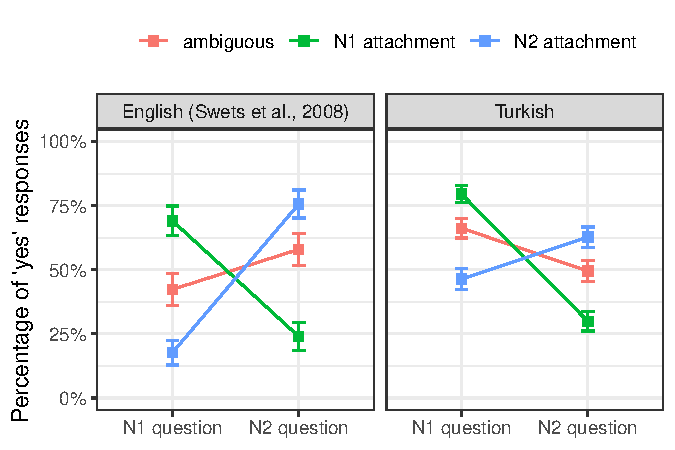
\includegraphics[width=7.5cm]{./figures/avg_perc.pdf}
\caption{Average percentages of \textit{'yes'} responses by attachment condition (color) and question type (x-axis). Error bars indicate 95\% within-subject CIs.}
\label{avg_perc}
\end{figure}

The average percentages of \textit{'yes'} responses in figure \ref{avg_perc} indicate a substantial number of errors in unambiguous experimental conditions in both experiments, such as \textit{'no'}-responses to N1 questions and \textit{'yes'}-responses to N2 questions about N1 attachment sentences.

The average accuracy in answering questions about unambiguous sentences was $79\%$ $(SE=1.3)$
% N1: 72.6 (1.3); N2: 79.0 (1.2)
in Swets et al.'s English experiment, and $66.5\%$ $(SE=2.5)$
% N1: 74.8 (2.3); N2: 58.2 (2.6)
in our Turkish experiment.

The responses in the ambiguous attachment conditions indicate an N2 attachment preference in the English as $58\%$ $(SE=2.1)$ of the response were compatible with N2 attachment (\textit{'yes'} responses to N2 questions and \textit{'no'} responses to N1 questions). Meanwhile, the Turkish data indicated an N1 preference as $58\%$ $(SE=1.9)$ of the question responses were compatible with an N1 interpretation of the sentence. In both cases, the preferred attachment option is \textit{local}, i.e., adjacent to the RC and is consistent with prior research.

%Although this paradigm differs somewhat from the experiments discussed in the introduction, the differences are minor, and both presumably reflect RC attachment preferences.
%
Even though the estimates of the magnitude of the attachment preference are coincidentally equal, the magnitude of the preference for local attachment may not be. This is due to the presence of a substantial number of erroneous responses in unambiguous conditions in both experiments. Their presence indicates a substantial number of \textit{guessing trials}, and thus suggests that not all N1- or N2-compatible responses in ambiguous indicate that the participant has successfully formed an N1- or N2 attachment interpretation of the sentence as they may have been generated by the same extraneous cognitive process that generates erroneous responses in the unambiguous attachment conditions.

The problem is exacerbated by the fact the response accuracy is particularly low in the N2 attachment condition in Experiment 2 ($58.2\%$). A possible reason for this is that even on trials resulting in an N2 interpretation, the parser always attempts to construct an N1 attachment structure first because, in Turkish, unlike in English, potential attachment sites are processed sequentially after the relative clause has already been processed. 
As a result, the presence of a discarded alternative N1 attachment structure \citep[e.g.,][]{Staub:2007} could interfere with the retrieval of the correct structure during question answering in N2 attachment conditions.
If, as a result of retrieval failure, participants resort to guessing, we would expect to observe a substantial number of erroneous responses following N2 attachment sentences or ambiguous sentences which were ultimately disambiguated towards N2 attachment.
% NOTE: I feel like these above-mentioned errors should be predominantly 'yes' responses. This can probably be tested by yet another model?

In the next section, we present two models of erroneous responses and then use them to estimate the magnitude of the actual strength of the attachment preference.


\section{MPT Models of Question-Answering and Attachment}

In accounting for the influence of extraneous cognitive processes, we considered two mechanisms that may generate erroneous question responses, and implemented both as multinomial processing tree (MPT) models \citep{BatchelderRiefer:1999}. In the following sections, we will use the model with the better empirical fit to obtain less biased estimates of the attachment preferences in the ambiguous conditions. 

MPT models offer a way to formalize hypotheses about how a mixture of several latent processes generates a categorical response 
\citep[cf.][ for an overview]{ErdfelderEtAl:2009}. 
That is, under the assumption that different sequences of events may occur on different trials, 
the latent processes hypothesized to be involved in processing are represented as a probability tree, with each path through the processing tree corresponding to unique combinations of cognitive processes which give rise to a particular response, along with the probabilities of each path.
Importantly, this formalization provides a framework in which the probabilities of relevant latent processes can be estimated. We will use them to estimate the magnitude of the RC attachment preference in Turkish and English.

% Erdfelder et al., 2009 

% ... quite useful as measurement models, but not necessarily mechanistic models, 

%The simplest model we can use for that are called multinomial processing tree models and allow us to specify that each participant's responses are essentially a mixture of 'informed responses' and 'uninformed random button presses', and we can estimate the true preference by factoring out the bias introduced by random button presses.



\subsection{Model 1}


The first mechanism we considered as a potential explanation for erroneous responses is that participants sometimes fail to attend to or successfully process the stimulus or the comprehension question and simply press a random button. We hypothesize that this may happen due to inattentiveness, careless responding,
distractions in the environment, mind-wandering \citep[e.g.,][]{Smallwood:2011}, (temporary) fatigue, or
failure to allocate sufficient processing resources towards the experimental task. We will subsume all of these factor under the umbrella term \textit{inattentiveness}.

The failure to process the stimulus is assumed to affect all three attachment conditions to the same degree. When participants do successfully comply with the task, they always respond to comprehension questions correctly in unambiguous conditions, while in ambiguous conditions, they sometimes adopt an N1 attachment interpretation of the sentence, and sometimes an N2 attachment, and answer comprehension questions in accordance with the adopted disambiguation of the ambiguous structure. 


\begin{center}
\begin{figure}[h!]
\noindent
\hspace*{-.7in}
\begin{scriptsize}
\begin{forest}
for tree = {
% nodes
    draw, 
    align=center,
    minimum height=5ex,
    minimum width=3em,
    font=\linespread{0.84}\selectfont,
% tree
    grow'=0,
    parent anchor=east,
    child  anchor=west,
    s sep = 4mm,    
    l sep = 12mm, 
% edge
    edge = {semithick},
% level styles
if level = 0{}{rounded corners=2ex},
where n children=0{tier=level, sharp corners}{calign=edge midpoint},
% edge labels
EL/.style={edge label={node [pos=0.5, fill=white,
                             font=\scriptsize\sffamily,
                             inner sep=2pt] {$#1$}}
                    }
            }% end for tree
[,coordinate
  [N1\\ attachment\\ condition,no edge
        [attentive\\ state, EL=a
            ['N1\\ response']
        ]
        [inattentive\\ state, EL=1-a,
            ['yes'\\ response, EL=g ]
            ['no'\\ response, EL=1-g]
        ]
  ]
  [N2\\ attachment\\ condition,no edge
        [attentive\\ state, EL=a
            ['N2\\ response']
        ]
        [inattentive\\ state, EL=1-a,
            ['yes'\\ response, EL=g ]
            ['no'\\ response, EL=1-g]
        ]
  ]
  [ambiguous\\ attachment\\ condition,no edge
        [attentive\\ state, EL=a
            [N1\\ attachment, EL=h
                ['N1\\ response']
            ]
            [N2\\ attachment, EL=1-h
                ['N2\\ response']
            ]
        ]
        [inattentive\\ state, EL=1-a,
            ['yes'\\ response, EL=g ]
            ['no'\\ response, EL=1-g]
        ]
  ]
]
\end{forest}
\end{scriptsize}

\caption{An MPT model of question answering with equal error rates for (i) N1 attachment, (ii) N2 attachment, and (iii) ambiguous sentences. }
\label{fig:mpt1}
\end{figure}
\end{center}

The assumptions of this account are illustrated in figure \ref{fig:mpt1}. 
The processing tree at the top illustrates how events during the processing of an N1 attachment sentence can unfold: On any given N1 attachment trial, a participant may be in an attentive state (with probability $a$) or an inattentive state (with probability $1-a$).
If the participant is in an attentive state throughout the trial (i.e., during reading and question answering), they will form a memory trace of the sentence they read, and later use it to correctly answer a comprehension question. This is illustrated in the top branch of the N1 attachment condition schematic in figure \ref{fig:mpt1}, where \textit{'N1 response'} stands for \textit{'yes'} responses to N1 questions and \textit{'no'} responses to N2 questions.

If the participant is in an inattentive state at any point during the trial (i.e., during reading or question answering), they will either fail to form a memory trace of the sentence they read or will fail to use it to answer the comprehension question. On those occasions, they will respond \textit{'yes'} with probability $g$, and \textit{'no'} with probability $1-g$. This is illustrated in the bottom branch of the N1 attachment condition MPT schematic in figure \ref{fig:mpt1}.



As a result of these assumptions, the probability of a \textit{'yes'} response in the N1 attachment condition is as given in equation \ref{eq:m1pN1}, where $I_{N1}$ (as in eq. \ref{eq:I_N1}) is an indicator variable which is $1$ for N1 comprehension questions (such as \textit{'Did N1 do RC?'}) and $0$ for N2 comprehension questions such (as \textit{'Did N2 do RC?'}).

\vspace{-0.5cm}
\begin{equation}
        I_{N1} = 
\begin{cases}
    1, & \text{for trials with N1 questions }\\
    0, & \text{for trials with N2 questions}
\end{cases}
    \label{eq:I_N1}
\end{equation}

\vspace{-0.25cm}
\begin{equation}
    p_{Y|N1} = a \cdot I_{N1} + (1-a) \cdot g
    \label{eq:m1pN1}
\end{equation}

The processing assumptions for the N2 attachment (middle, figure \ref{fig:mpt1}) condition and the ambiguous condition  (bottom, figure \ref{fig:mpt1}) follow a similar logic, with the probability of a \textit{'yes'} response given by equations \ref{eq:m1pN2} and \ref{eq:m1pAmb}. 

\vspace{-0.5cm}
\begin{equation}
    p_{Y|N2} = a \cdot ( 1 - I_{N1} ) + (1-a) \cdot g
    \label{eq:m1pN2}
\end{equation}

An important assumption about the hypothesized processes in ambiguous attachment conditions is that when readers are in an attentive state, they disambiguate ambiguous sentences either towards an N1 interpretation (with probability $h$) or an N2 interpretation (with probability $1-h$). We make no assumptions about whether that happens during reading or at the question answering stage.
% ... only yes responses as the only alternative

\vspace{-0.5cm}
\begin{equation}
    p_{Y|A} = a \cdot   [ h  \cdot I_{N1} + (1 - h) \cdot (1-I_{N1}) ]  + (1-a) \cdot g 
    \label{eq:m1pAmb}
\end{equation}
\vspace{0.1cm}


Importantly, we make no assumptions as to what may bring on inattentiveness and whether it occurs predominantly during reading or question answering. The key assumption of this account, however, is that this process affects all attachment conditions to the same degree. 


\subsection{Model 2}
 
The second model included an additional possible source of erroneous responses that may not affect all attachment conditions equally. 
We hypothesized that, as observed in the unambiguous conditions of Experiment 2, one of the two interpretations (N1 or N2 attachment) could be more prone to failure, in that it may be less likely to be successfully created during reading, or less likely to be successfully recalled during question answering. 
%A possible reason for such a difference in both experiments is that RC attachment is disambiguated via anaphor binding. Therefore, it is possible, in principle, that the preferred interpretation is usually attempted first, even in dispreferred attachment conditions, before that interpretation is rejected, and the correct dispreferred interpretation is constructed. Moreover, the fact that Turkish relative clauses are available before 

\begin{center}
\begin{figure}[h!]
\hspace*{-0.7in}
\begin{scriptsize}
\begin{forest}
for tree = {
% nodes
    draw, 
    align=center,
    minimum height=5ex,
    minimum width=3em,
    font=\linespread{0.84}\selectfont,
% tree
    grow'=0,
    parent anchor=east,
    child  anchor=west,
    s sep = 4mm,    
    l sep = 12mm, 
% edge
    edge = {semithick},
% level styles
if level = 0{}{rounded corners=2ex},
where n children=0{tier=level, sharp corners}{calign=edge midpoint},
% edge labels
EL/.style={edge label={node [pos=0.5, fill=white,
                             font=\scriptsize\sffamily,
                             inner sep=2pt] {$#1$}}
                    }
            }% end for tree
[,coordinate
  [N1\\ attachment\\ condition,no edge
        [recollection\\ certainty, EL=r_{1}
            ['N1\\ response']
        ]
        [recollection\\ uncertainity, EL=1-r_{1},
            ['yes'\\ response, EL=g ]
            ['no'\\ response, EL=1-g]
        ]
  ]
  [N2\\ attachment\\ condition,no edge
        [recollection\\ certainty, EL=r_{2}
            [N2\\ response]
        ]
        [recollection\\ uncertainity, EL=1-r_{2},
            ['yes'\\ response, EL=g ]
            ['no'\\ response, EL=1-g]
        ]
  ]
  [ambiguous\\ attachment\\ condition,no edge
      [N1\\ attachment,EL=h
            [recollection\\ certainty, EL=r_{1}
                [N1\\ response]
            ]
            [recollection\\ uncertainity, EL=1-r_{1},
                ['yes'\\ response, EL=g ]
                ['no'\\ response, EL=1-g]
            ]
      ]
      [N2\\ attachment,EL=1-h
            [recollection\\ certainty, EL=r_{2}
                [N2\\ response]
            ]
            [recollection\\ uncertainity, EL=1-r_{2},
                ['yes'\\ response, EL=g ]
                ['no'\\ response, EL=1-g]
            ]
      ]
  ]
]
\end{forest}
\end{scriptsize}
\caption{An MPT model of question answering with different error rates for N1 attachment and N2 attachment processes.
}
\label{fig:mpt2}
\end{figure}
\end{center}

We formalized the assumption of different error rates associated with N1 and N2 attachment in the model in figure \ref{fig:mpt2}. The hypothesized structure of unambiguous N1 and N2 attachment trials is similar to Model 1 in figure \ref{fig:mpt1}. Each attachment process (N1 and N2 attachment) is associated with a probability of complete recollection certainty ($r_1$ and $r_2$, respectively) which reflects the probability that the correct sentence structure is (i) constructed during reading and (ii) later correctly recalled during the question answering phase. If the correct sentence structure is constructed and recalled, participants respond in accordance with the structure they constructed. Otherwise, they select a random response, i.e., \textit{'yes'} with a probability of $g$ and \textit{'no'} with a probability of $1-g$. The probability of a \textit{'yes'} response for all attachment conditions is given in equations \ref{eq:m2pN1}, \ref{eq:m2pN2}, \ref{eq:m2pAmb}.


In the ambiguous condition (figure \ref{fig:mpt2}, bottom), the recollection certainty and recollection uncertainty nodes are nested under the RC attachment nodes because the probabilities of the recollection certainty and uncertainty states depend on which RC attachment was chosen.

\begin{equation}
p_{Y|N1} = r_1 \cdot I_{ N1 } + (1-r_1) \cdot g
\label{eq:m2pN1}
\end{equation}
\vspace{-0.5cm}
\begin{equation}
p_{Y|N2} = r_2 \cdot (1 - I_{N1}) +  (1-r_2) \cdot g
\label{eq:m2pN2}
\end{equation}
\vspace{-0.5cm}
\begin{equation}
p_{Y|A} =  h  \cdot p_{Y|N1} + (1-h) \cdot p_{Y|N2}
\label{eq:m2pAmb}
\end{equation}


Importantly, Model 2 (fig. \ref{fig:mpt2}) subsumes Model 1 (fig. \ref{fig:mpt1}) and therefore does not exclude the influence of an additional attention-related processes that affect all attachment conditions equally. 
This is because it can be re-parameterized as $(1-r_1) = (1-a) + (1-r_1')$ and $(1-r_2) = (1-a) + (1-r_2')$, such that the guessing rates in N1 and N2 attachment conditions, $(1-r_1)$ and $(1-r_2)$, can be interpreted as the sums of the attention-related guessing rate $(1-a)$ and the condition-specific guessing rates $(1-r_1')$ and $(1-r_2')$.


\section{Method}

We implemented both MPT models\footnote{All code has been made available at \url{https://git.io/JODKF}}
in \textit{brms} and \textit{rstan} \citep{R-brms, rstan} in R \citep{R-base} according to equations \ref{eq:m1pN1}-\ref{eq:m2pAmb}. We fitted the models to each experiment separately, using $4$ MCMC chains with $1,000$ warm-up and $3,000$ post-warm-up iterations.
For the sake of computational convenience, we estimated all model parameters on the logit scale, and in the following, we will use $\theta'$ to refer to the logit-transform of any parameter $\theta$.

We used mildly informative Gaussian priors for all logit-transformed population parameters in both models: $h', g' \sim N(0,1)$, and $a, r_1, r_2 \sim N(0,1)$.

To account for individual differences in all parameters, we used hierarchical models with by-subject intercepts for all parameters, where each participant $k$'s responses were modeled as a function of population-level parameters $\theta$ with subject subject-level adjustments $\delta_{\theta,k}$, with $\theta_k' = \theta' + \delta_{{\theta'},k}$, where the by-subject adjustments are  distributed as $\delta_{{\theta'},k} \sim N(0, \sigma_{\theta'})$.

% ($a_k, h_k, g_k, r_1_k, r_2_k$), where $k$  
% to-do: link to the anonymized github repo
% The code and data can be found in the git repo here:

\section{Model Comparison}

Figures \ref{post_pred_ahg} and \ref{post_pred_r1r2hg} show the average percentages of \textit{'yes'} responses by experiment (circles and connecting lines) alongside 95\% posterior predictive intervals generated by, Model 1 and 2, respectively (error bars).

\begin{figure}
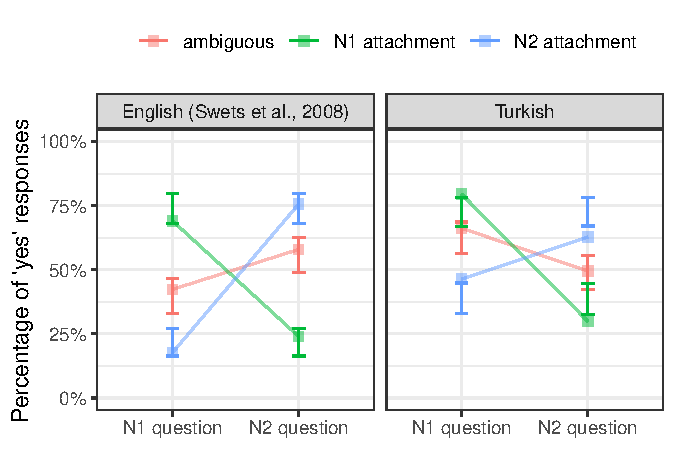
\includegraphics[width=7cm]{./figures/post_pred_ahg.pdf}
\caption{Average percentages of \textit{'yes'} responses in the experiments, and $95\%$ posterior prediction intervals based on Model 1 by attachment condition and question type.}
\label{post_pred_ahg}
\end{figure}

\begin{figure}
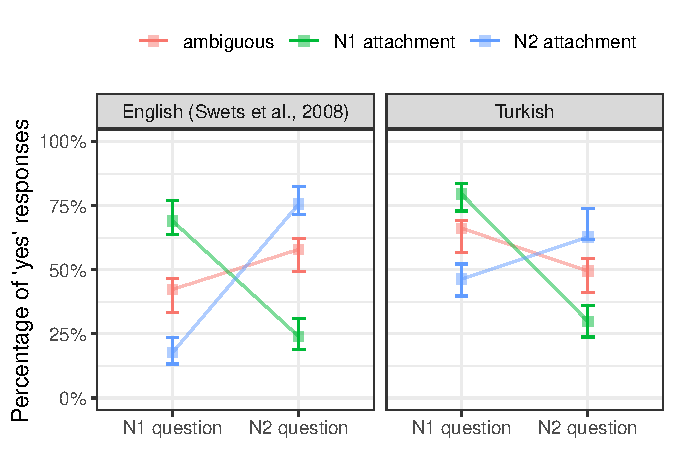
\includegraphics[width=7cm]{./figures/post_pred_r1r2hg.pdf}
\caption{Average percentages of \textit{'yes'} responses in the experiments, and $95\%$ posterior prediction intervals based on Model 2 by attachment condition and question type.}
\label{post_pred_r1r2hg}
\end{figure}

Figure \ref{post_pred_ahg} shows that although Model 1 could approximate the experimental findings 
%presented in fig. \ref{avg_perc}
%to some degree, 
it systematically overestimated the proportion of responses compatible with the preferred RC attachment (N2 in English, N1 in Turkish) in both unambiguous conditions: For example, in the N1 attachment condition in English, the number of \textit{'yes'} responses to N1 questions and \textit{'no'} responses to N2 questions were slightly overestimated. Similarly, in the N2 attachment condition in Turkish, the model underestimated the percentages of \textit{'yes'} responses to N1 questions and \textit{'no'} responses to N2 questions. Figure \ref{post_pred_r1r2hg} shows that Model 2 appeared to have fewer systematic deviations, and appeared to fit the data quite well.

In order to compare the models more formally, we using PSIS-LOO-CV \citep{loo} to compute
each model's expected log pointwise predictive density (ELPD). ELPD provides an estimate of the model's out-of-sample performance and thus penalizes additional model flexibility, which puts Models 1 and 2 on an equal footing although Model 2 has more parameters.
Table \ref{tab:model_comp} shows the ELPD estimates ($\Delta\widehat{elpd}$), as well as the differences between models in $\Delta\widehat{elpd}$ along with their respective standard errors. Larger values indicate better performance.

Both $\Delta\widehat{elpd}$ estimates are relatively large relative to their standard errors, and thus point towards Model 2 having better out-of-sample performance.
This finding suggests that the two attachment processes are affected by the error-generating process to different degrees.



\begin{table}
\centering
\begin{tabular}{lcc}
        & English & Turkish \\
\hline
        & $\widehat{elpd}$ & $\widehat{elpd}$ \\
\hline
model 1 & $-511.3$ $(18.1)$ & $-796.4$ $(15.0)$ \\
model 2 & $-469.4$ $(14.8)$ & $-750.5$ $(13.5)$ \\
\hline
 &  &  \\
 & $\Delta\widehat{elpd}$ & $\Delta\widehat{elpd}$ \\
\hline
model 2-1 & $41.9$ $(11.6)$ & $45.9$ $(9.3)$
\end{tabular}
\caption{Estimates of expected log pointwise predictive density ($\widehat{elpd}$) by model for each experiment and differences between model $\widehat{elpd}$s. Standard errors in brackets. }
\label{tab:model_comp}
\end{table}



\section{Results}

Having established Model 2 as an adequate model of RC attachment in the context of question-answering, we used its parameter estimates to understand the pattern of responses in the experimental data: Figure \ref{estimates_r1r2hg} shows the Model 2 population parameter estimates for both experiments as well as 95\% credible intervals for all four parameters. In addition to the difference in the guessing bias $g$ between experiments, it also shows a lot of uncertainty in the estimates of the attachment parameter $h$, which represents the probability with which the parser adopts an N1 attachment interpretation over an N2 attachment structure in ambiguous attachment conditions. 
Both estimates of the N1 attachment probability have rather wide credible intervals, with $42\%$ $(CrI=[30; 55])$ for the English experiment and $48\%$ $(CrI=[24; 70])$ for the Turkish experiment. While the estimate for English is consistent with weak evidence for an N2 attachment preference, the estimate for Turkish indicates no clear preference.


\begin{figure}
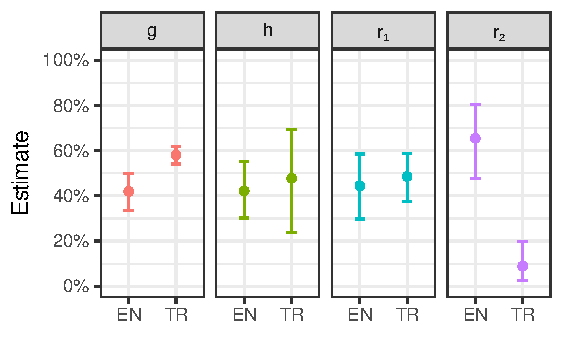
\includegraphics[width=7cm]{./figures/estimates_r1r2hg.pdf}
\caption{Population parameter estimates and 95\% credible intervals for all four parameters of Model 2 ($g, h, r_1, r_2$) for both experiments, English (EN) and Turkish (TR). }
\label{estimates_r1r2hg}
\end{figure}

The explanation for the surprising absence of evidence for an N1 attachment preference in the parameter $h$ in Turkish lies in the the substantial difference between the successful recall probabilities $r_1$ ($49\%$, $CrI=[38; 59]$) and $r_2$ ($9\%$, $CrI=[3; 20]$), which indicate that N1 interpretations were successfully processed and recalled with a higher probability than their N2 counterparts.
According to the assumptions of Model 2, this leads to a question response pattern which appears to suggest an N1 preference even when there isn't one ($h=0.5$): When participants decide to adopt an N1 interpretation, their question responses indicate N1 attachment on most trials -- sometimes due to successful recall of the N1 interpretation, and at other times as a result of guessing. When participants decide to adopt an N2 interpretation, however, they fail to recall the correct interpretation most of the time, and thus engage in guessing. Importantly, guesses result in N1 responses $50\%$ of the time, since questions about N1 and N2 interpretations are balanced. As a result, a substantial difference between $r_1$ and $r_2$, such that $r_1 < r_2$ will lead to more N1 responses than N2 responses to questions about ambiguous sentences because N1 interpretations are more successfully recalled, even if ambiguous sentences are assigned N1 interpretations only $50\%$ of the time.

Whatever the source of higher error rates in the N2 attachment conditions in the Turkish experiment is, our MPT analysis suggests that what appears as a weak N1 attachment preference in our Turkish experiment is actually a consequence of a large number of \trials{guessing trials} associated with N2 attachment.
In sum, our analysis shows that (i) the N2 attachment preference in the English experiment appears to hold up even when guessing trials are taken into account, and (ii) that what appears to be an N1 attachment preference in Turkish is readily explained by the processing difficulty associated with processing and recalling N2 attachment structures in Turkish.


%\begin{figure}
%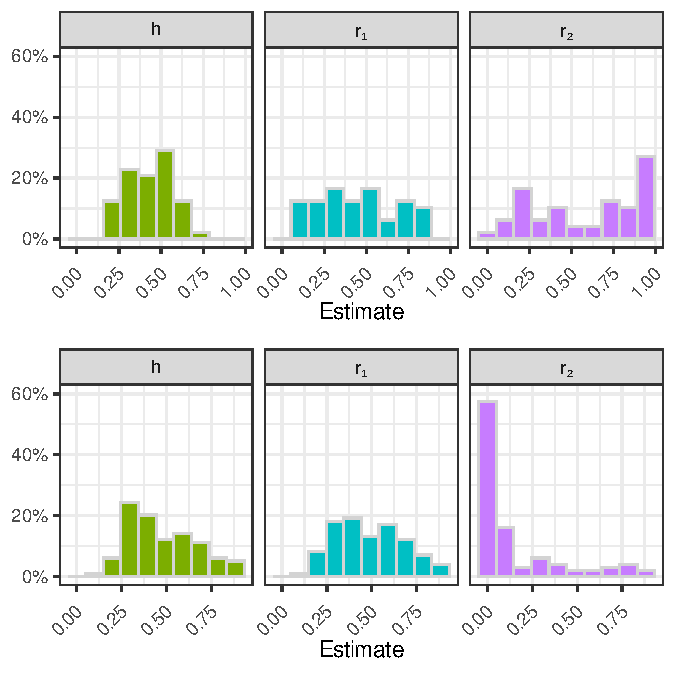
\includegraphics[width=7cm]{./figures/estimates_r1r2hg_bysubj.pdf}
%\caption{Histogram of by-participant MAP parameter estimates ($\theta + \delta_{\theta,k}$) for the parameters $h$, $r_1$, $r_2$ for the English (top) and Turkish (bottom).}
%\label{estimates_r1r2hg_bysubj}
%\end{figure}


\section{Summary}

Based on the assumption that readers sometimes do not allocate the required amount of attention to the task they are performing, we have discussed a previously neglected source of bias and variability that may affect studies of attachment preferences and of interpretation preferences more generally. We attempted to account for the role of guessing as a strategy used in answering comprehension questions when the answer is not known. We argue that understanding the role of guessing in discrete choice tasks is crucial because data consisting of responses to comprehension questions where participants sometimes fail to arrive at a full interpretation of the structure may be confounded. To this end, we proposed an MPT-based analysis method that allows to de-confound parameters of theoretical importance from nuisance parameters such as the guessing rate. We tested two variants of the MPT-based model on experimental data from English and Turkish, and demonstrated that this method can provide further insight into the processes underlying participants' answering behavior as well as their attachment preferences. 



%Well, it's because they several sources of variation which the MPT can help us separate. Importantly, using averages to estimate attachment preferences amounts to just using model 1 with a=1, which is clearly an inadequate model, given that model 1 with a free $a$ parameter is already quite bad, and given that the estimates of $r_1$ and $r_2$ are quite far away from 1.

%- Talk about how this method might be assumption-ladden, but so is the method of using averages - and those are definitely wrong.



%\section*{Acknowledgements}
%We would like to thank Müge Tuncer for her help with the design of the Turkish experiment, as well as Kadernur Akpınar, Hande Sevgi and Utku Türk for their assistance with the experimental stimuli.
%We would also like to thank Benjamin Swets for kindly sharing the \citet{SwetsEtAl:2008} experimental data, as well as three anonymous reviewers for their very helpful feedback.

\bibliography{custom} % anthology,
\bibliographystyle{acl_natbib}

%\appendix
%\section{Example Appendix}
%\label{sec:appendix}
%This is an appendix.

\end{document}
